\documentclass{article}
\usepackage[utf8]{inputenc}

\title{CSE 222A PROJECT - GROUP 6}

\author{Sreejith Unnikrishnan, Stanislav Mushits, Amit Borase, Ritvik Jaiswal }
\date{November 4 2015}

\usepackage{natbib}
\usepackage{graphicx}

\begin{document}

\maketitle

\begin{center}
\textbf{Milestone report}
\end{center}


\section{Project Topic}
The objective of our project is to verify the varys scheduler\cite{varys} and associated performance improvement in a data center environment. 

\section{Progress So Far}
As a part of this goal, we have completed the following tasks.

\begin{itemize}
\item Analyse and select various frameworks and technologies to be used.
\item Automate the development and simulation environment setup on the allotted virtual machines.
\item Study and analyse various network topologies prevalent in data center environments. Chose fat-tree topology for its increasing popularity in data center solutions.
\item Automate the deployment of the fat-tree topology that can be configured as per need.
\item Generate sample map-reduce traces that simulates the map-reduce traffic patterns over the network.
\item Segregate such network traces into set of per-host schedulable network events.
\item  Develop an actor program that runs on every hosts. It listens for launch signals from controllers, and based on current host's network traces and additional configuration files, it simulates network traffic originating from current host. Actor can work in two modes, in traditional mode (no coflow scheduling) and varys mode (coflow scheduled using varys). Currently it works sequentially and lacks parallelization.
\item Develop a populator program that synchronizes various map-reduce schedule times by issuing launch commands to hosts in the network.

\end{itemize}

\subsection{System structure}
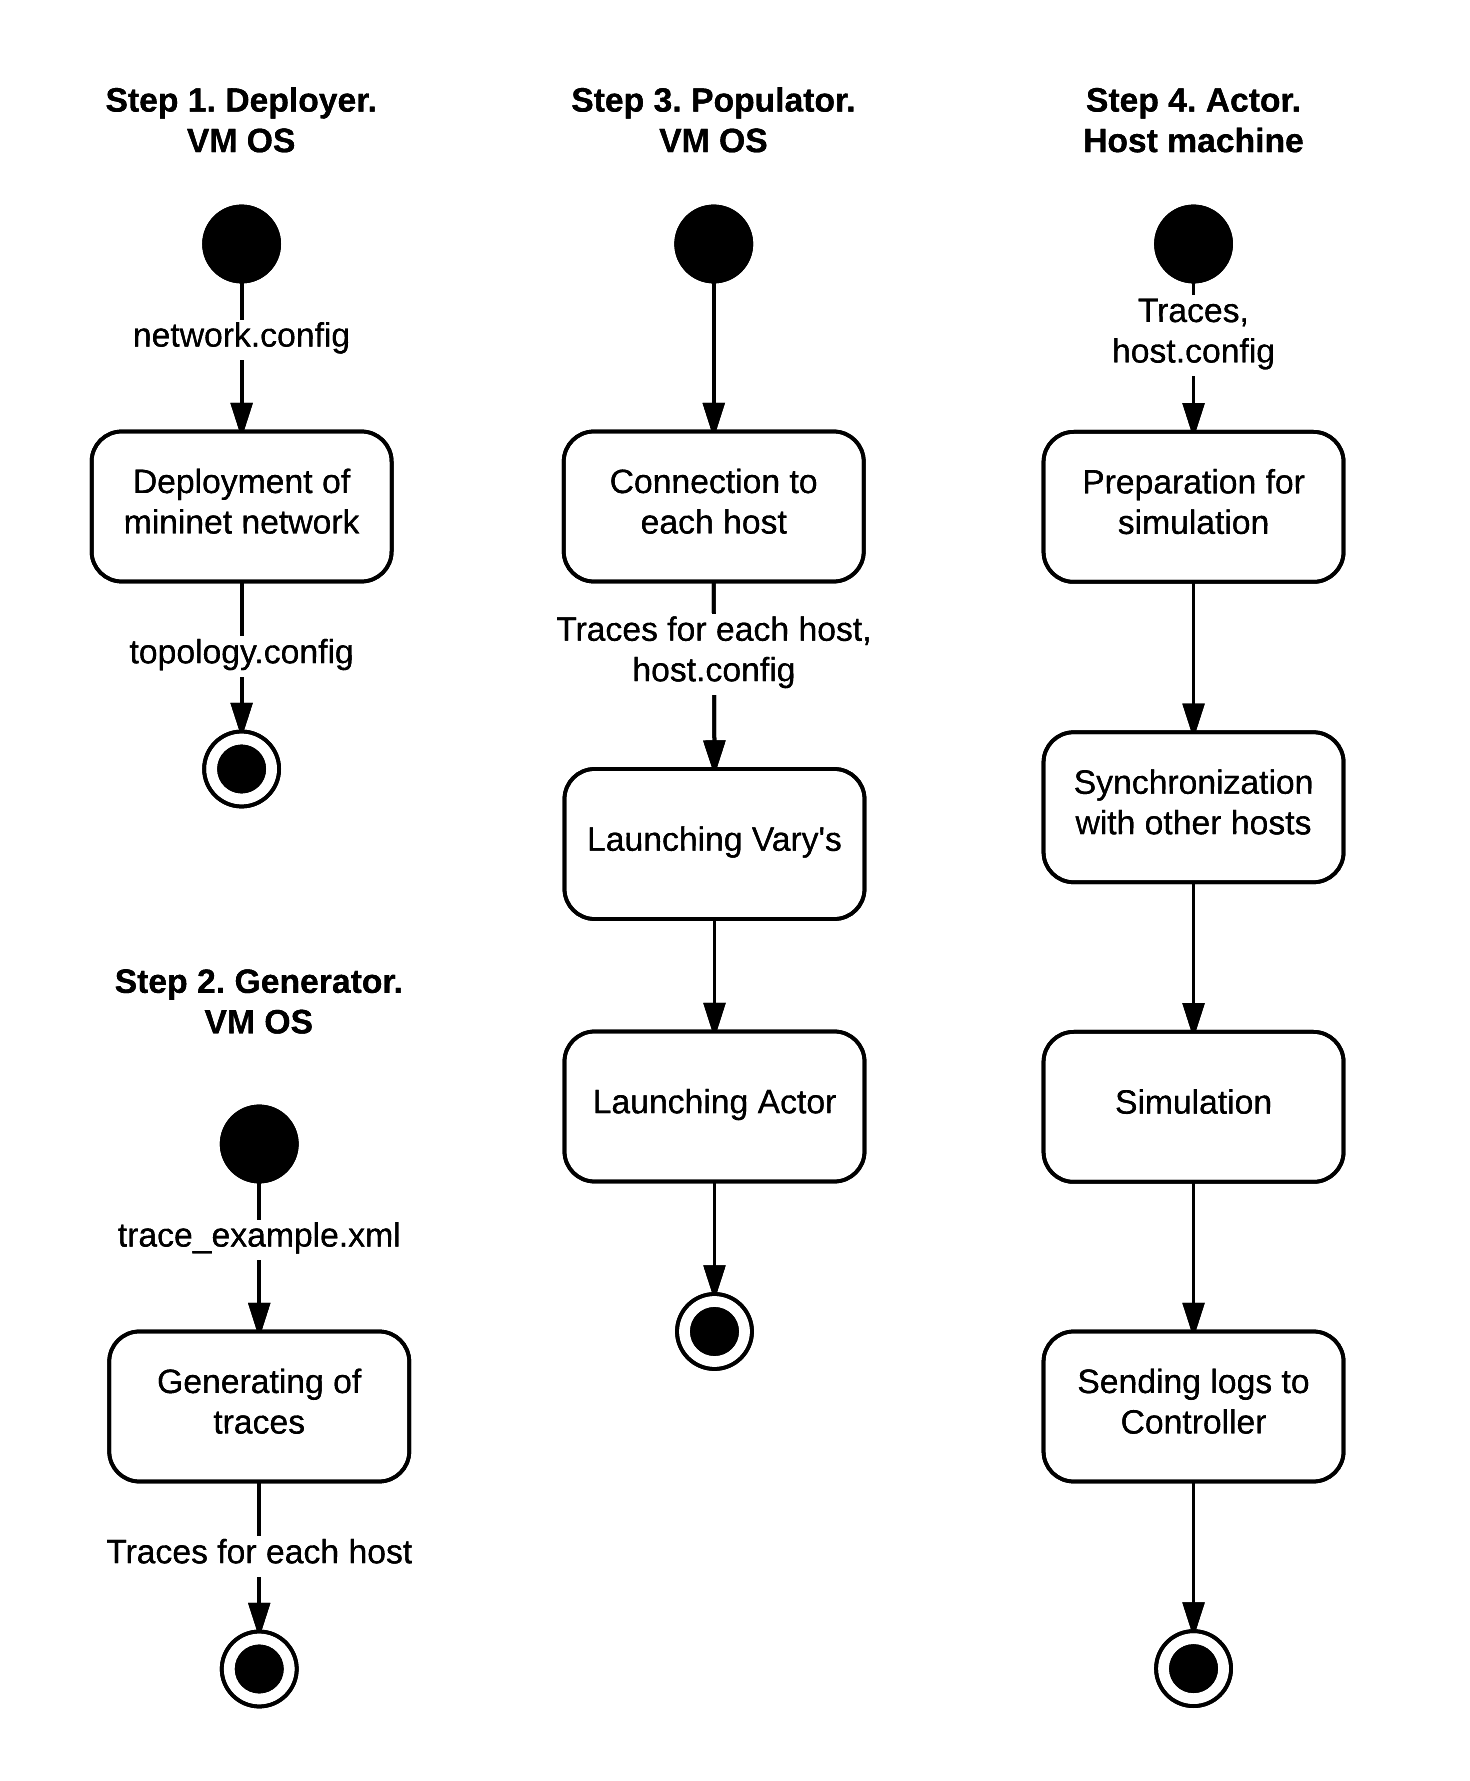
\includegraphics[scale = 0.75]{flow_diagram}
\begin{itemize}
\item The deployer program takes network.config file and creates the required topology.
\item The trace generator generates segregated trace files for each host.
\item The populator program runs on the VM host and launches varys scheduler along with actor program on each host.
\item The actor machine gathers per host trace file, host.config and runs the simulation. It also probes for various network parameters and logs the results.
\end{itemize}

\subsection{Challenges faced}
One of the main challenges was to adopt a topology that efficiently simulates a data-center network. To make our simulation more realistic, we studied various papers on recent data-center advances, the ones discussed during classes and beyond. We selected fat tree topology for our simulations since it is widely used currently and provides efficient bisection bandwidth for all the hosts in the data-center. We use an open source tool FNSS \cite{fnss}, that provides effective API`s to model fat tree topology for data-centers. However we need to run Varys scheduler on each of the hosts. That means we would have to go with mininet. So to benefit from FNSS and mininet both, we generate topology using FNSS and instantiate it on the mininet.

Another challenging task is to model and generate network traffic that closely mimics the real-life map-reduce deployments. To understand the traffic pattern we read through various papers including 'Inside the Social Network's (Datacenter) Network' co-authored by Prof. Porter \cite{facebook}. This helped us to understand fundamental differences between web traffic pattern and map reduce jobs. We created a network traces for simulations, in accordance with these traffic patterns.

\section{Next steps}

Below are the set of pending tasks in the project:

\begin{itemize}
\item Improve actor and controller program by incorporating multiple connections and data parallelisation.
\item Integrate individual pieces together to bring up the complete setup.
\item Using sample network schedules, verify that the setup is up and running.
\item Run the tests with realistic network traces, with actor program running in varys scheduler mode. Collect and analyze the results.
\item Run the same set of tests with actor program running without involving varys scheduler. Collect and analyze the results.
\item Compare and verify the obtained results for various network parameters.
\end{itemize}

\section{Graphical Analysis}
We plan to collect data-points such as coflow completion times, coflow sizes, coflow fractions, job completion times and job completion percentages for map-reduce traffic patterns, followed by analyze such data to report below set of graphs.
\begin{itemize}
\item Comparison of coflow completion times with varying coflow sizes, with and without varys scheduler for map reduce traffic. We evaluate whether varys scheduler improves the performance of such traffic patterns, if yes then to what extent. The X-axis will plot the Coflow completion time while Y-axis will plot factor of improvement.
\item Comparison of coflow completion times with fraction of the coflows involved, with and without varys scheduler running. The X-axis will plot the coflow completion times and the Y-axis will plot the fractions of coflows involved.
\item Comparison of Job completion times, with and without varys scheduler for map reduce traffic. This graph will show whether or not the varys scheduling results in the improvement of job completions times. The X-axis of such graph will plot the job completion times and the Y-axis will plot the factor of improvement.
\item Comparison of percentage of coflows that met their deadlines, with and without varys scheduler for map reduce traffic. This graph will show whether or not the varys scheduling results in the increased number of coflows meeting their deadlines. The X-axis of such graph will plot the percentage of coflows meeting their deadlines and the Y-axis will plot the deadline times.
\item Comparison of percentage of coflows that met their deadlines with the number of concurrent coflows, with and without varys scheduler for map reduce traffic. This graph will show the effect of coflow concurrency on the percentage of coflows meeting their deadlines. The X-axis of such graph will plot the number of concurrent coflows involved and the Y-axis will plot the percentage of coflows meeting their deadlines.
\end{itemize}


\bibliographystyle{plain}
\begin{thebibliography}{10}
\bibitem{varys}
Efficient Coflow Scheduling with Varys, Mosharaf Chowdhury, Yuan Zhong, Ion Stoica, ACM SIGCOMM, 2014.

\bibitem{fnss}
Fast Network Simulation Setup \textit{https://github.com/fnss/fnss/}

\bibitem{repo}
Team 06 Github Repo \textit{https://github.com/ucsdcse222a/group6}

\bibitem{facebook}
Inside the Social Network’s (Datacenter) Network - SIGCOMM 2015
\textit{Arjun Roy, Hongyi Zeng, Jasmeet Bagga, George Porter, and Alex C. Snoeren}

\end{thebibliography}

\end{document}

